\chapter{Introduction}
\label{sec:intro}

\subsection*{Why we study few nucleon systems}

The study of light nuclei and their reactions has been serving as an easy way to investigate particles in nuclei and
the forces between them for decades. A convenient way to proceed may be to study the interaction of a nucleus with
other nuclei, particles, or electroweak probes such as electrons, photons, muons, pions, neutrinos, and hyperons.
In most cases, the study of elastic or inelastic scattering is possible. This can be done either theoretically or by
performing relevant experiments to test if the theory works. It should be taken into account that nuclear 
interactions may be
caused by different fundamental forces, including strong, weak, or electromagnetic
interactions. This depends on the type of particle being scattered and the target of the reaction
and requires different theoretical approaches.
Of course gravitational force is also in the game but due to its weakness it is 
usually omitted in the nuclear physics. 

In the past many experimental efforts have been undertaken and
experimentalists have been interested in electromagnetic reactions involving light nuclei for decades.
There are experimental data from the second half of the 20th century 
(e.g. \cite{Skopik1974, Liuexp68, Kose1969MeasurementsOT, Kamae}) which are still 
useful for comparing theoretical predictions with experimental measurements.    
There are several facilities providing sources of gamma rays (both low- and high-energy)
and other particles that have been operating for decades and still enable experiments to be conducted.
Let us mention here such facilities as TUNL with HI$\gamma$S \cite{TUNL, TONCHEV2005170} or MAMI \cite{MAMI}. 
% NIKHEF \cite{NIKHEF} and others.

To accurately describe nuclear reactions, two important components of the Hamiltonian must be considered.
They are nuclear interactions and nuclear currents.
First of all, various nuclear forces may act on
the particles.

The strong nuclear force acts inside the nuclei and, among others, binds neutrons 
and protons together. The description of strong interactions is extremely
difficult as it deals not only with the nucleons themselves but also with their constituents: quarks
and gluons. \gls{qcd} is a modern theory
describing strong interactions, but, at the moment,
it is not applicable at low energies (e.a. at $Q^2 \lesssim 1 GeV^2$).
In such a situation, various approaches are emerging.
The most advanced is the
chiral effective theory and lattice calculation \cite{IOFFE2006232, BEANElaticce, Machleidt2011}.
In this work we will use the results of the first approach
and the corresponding model is described in Sec.~\ref{sec:formalism}.

A study of three- (and more) nucleon systems showed that
the strong \gls{2n} force is not efficient in describing
$N>2$ systems, thus a three-nucleon (3N) force (3NF) was introduced. The first applications of such
a force showed that it brings a
sizable contribution to observables and cannot be ignored \cite{GLOCKLE1982343}.
The contribution of the 3NF can be examined e.g. by
comparing binding energies of light nuclei calculated with
and without this part of the Hamiltonian, and with respect to experimental data.

For example, the binding energy\footnote{More precisely it is a ground state energy, but I follow commonly used mental shortcut.}
for $^3$H calculated with the \gls{av18} \gls{2n} potential 
without 3NF amounts to
$E_b(^3\mathrm{H}) = \SI{-7.628}{\mev}$ \cite{NoggaAV18}. There are different models that might add a 3NF
contribution to \gls{av18} (or other potentials). Using the Tucson-Melbourne (TM) model \cite{Tucson-Melbourne}
results in $E_b(^3\mathrm{H}) = \SI{-8.478}{\mev}$, and the Urbana IX \cite{Urbana3NF} 3NF provides us with
$E_b(^3\mathrm{H}) = \SI{-8.484}{\mev}$. Looking at the experimental value $E_b(^3\mathrm{H}) = \SI{-8.482}{\mev}$,
it is clear that the 3NF contribution makes the prediction much closer to the measurement.
Nevertheless, the parameters of the UrbanaIX
3NF were fitted to the experimental value for $^3\mathrm{H}$, so there is no surprise in good agreement.

However one can also check the binding energy for other nuclei, which were not used for the fitting.
The 2N force (2NF) binding energy for $^3$He
(calculated with \gls{av18}) is $E_b(^3\mathrm{He}) = \SI{-6.917}{\mev}$. The TM contribution makes it
$E_b(^3\mathrm{He}) = \SI{-7.706}{\mev}$, the Urbana IX gives $E_b(^3\mathrm{He}) = \SI{-7.739}{\mev}$, while the
experimental value is $E_b(^3\mathrm{He}) = \SI{-7.718}{\mev}$. One can see the importance of 3NF
contribution also for the $\alpha$-particle's ($^4\mathrm{He}$) binding energy:
the \gls{av18} alone gives
$E_b(^4\mathrm{He}) = \SI{-24.25}{\mev}$, while the \gls{av18} + TM leads to \SI{-28.84}{\mev},
the \gls{av18} + Urbana IX delivers $E_b(^4\mathrm{He}) = \SI{-28.50}{\mev}$,
and the experimental value is \SI{-28.30}{\mev}\cite{NoggaAV18}.

Whereas the first applications included only early simplified "realistic" 3N potential, the latter
investigations, based on more advanced models, fully confirmed above statements \cite{StoksPhysRevC49, AV18Wiringa}.
Within new models, the four-nucleon (4N) interaction was constructed to improve the description of
$^4\mathrm{He}$ \cite{NoggaPhysRevLett}.
A broader discussion of models of nuclear forces used in this thesis is given below.

The electromagnetic force appears between charged particles like protons, electrons, or pions.
That force acts also between charged particles and photons, so 
in photon- and electron- scatterings on the nuclei 
it is a necessary component of a description.
However, electromagnetic interaction between nuclei manifests mainly at very 
low energies or for specific kinematic configurations with two
protons having approximately equal momenta.
Thus it is skipped in the lowest-order analysis.

The main contribution of electromagnetic interaction 
to disintegration processes in hand is due to the current operator
describing photon-nucleon vertex and second-order processes.
The structure of the electromagnetic current has been investigated
in many works by numerous groups \cite{Carlson1997} but it was 
H.~Arenh\"{o}vel who performed a study of nuclear electromagnetic
current in the few-nucleon sector.
His long-term research, reviewed in \cite{ArenhovelPhotodisint1991}
% in his works
% \cite{Wilbois1993, ArenhovelLeid1995, ArenhovelLeid1998, Arenhvel2004} 
demonstrated various theoretical models applied to the deuteron photodisintegration.
He analyzed among others a nonrelativistic potential model,
a relativistic impulse approximation, and a relativistic meson-exchange model.
These models were used to calculate the differential cross section and various
polarization observables, which describe the probability
of the process occurring at different scattering angles, photon energies, spin directions, etc.

The calculated cross sections were then compared to experimental data, and it was
found that the relativistic meson-exchange model provided
the best agreement with the data at photon's energies up to $E_\gamma \approx \SI{100}{\mev}$.
At higher energies agreement is observed too but is getting worse.
This model includes the exchange of virtual mesons
between the interacting particles, which accounts for
the strong and electromagnetic forces between them.

Overall, Arenh\"{o}vel demonstrated the importance of including both strong interaction
and electromagnetic current operator in a description of the deuteron photodisintegration process,
and highlighted the need for accurate theoretical models to interpret experimental data.


The weak force is of great importance in the study of nuclear processes. One of the main roles of the weak force is to mediate 
negative  beta decay,
which is a process in which a neutron in a nucleus is converted into a proton, emitting an electron and an antineutrino. This process plays
a crucial role in the formation of elements in the universe, as it allows for the conversion of neutron-rich isotopes into more stable,
proton-rich isotopes. Additionally, the weak force plays a role in neutrino interactions with matter, which are of great interest in both
astrophysics and particle physics. In nuclear physics, weak interactions can also play a role in the decay of unstable nuclei, the
production of neutrinos in nuclear reactions, and the scattering of neutrinos off nuclei. The study of weak interactions is therefore an
essential component of the overall understanding of nuclear physics and the behavior of matter on the subatomic scale.
However, in the thesis, I stick with electromagnetic and strong processes.


\subsection*{Models of strong interaction used in the thesis}

In order to model the nuclear potential, physicists often use phenomenological
or semi-phenomenological approaches. It allows them to combine
theoretical knowledge about the studied processes and experimental findings.

% \tmp{?more}
Among many of such models, the \gls{av18} \cite{AV18Wiringa} force is one of the most
advanced and therefore is used in the current thesis.
To construct that \gls{nn} force, authors combine
% analytical electromagnetic and 
long-range one-pion-exchange part
with short-range phenomenological one and supplement them with electromagnetic corrections.
Free parameters were fitted to
the Nijmegen partial-wave analysis of $pp$ and $np$ data \cite{NijmegenPhysRevC.48.792}. 
Authors showed, that the \gls{av18} potential delivers good 
description of nucleon-nucleon scattering data ($\chi ^2/data = 1.08$ for around \num{4000} $pp$ and $np$ scattering data points) 
as well as deuteron properties (estimated binding energy is \SI{2.2247(35)}{\mev} vs experimental \SI{ 2.224 575(9)}{\mev} \cite{VANDERLEUN1982261}).

Weinberg's idea of using chiral symmetry to describe nuclear interactions at low
energies was first introduced in his papers published in 1990 and 1991 \cite{WEINBERG1990,WEINBERG1991}.
In these papers, Weinberg argued that the low-energy dynamics of nucleons
could be described using a chiral Lagrangian, which is the most general
Lagrangian consistent with chiral symmetry and its spontaneous breaking.
This Lagrangian is expressed in terms of nucleon and pion fields,
which are the degrees of freedom that become relevant at low energies.

The chiral Lagrangian is the starting point for the development of
the \gls{ceft}, which has become one of the
most advanced approaches to low-energy nuclear physics \cite{EpelHam2008}.
The use of the \gls{ceft} allows (at least in theory) for the calculation of nuclear properties
and reactions in a model-independent way.
It is also possible to
quantify the uncertainties associated with the calculation. One of the
key features of the \gls{ceft} is that it allows for the construction of
a nuclear potential, which can then be used in relevant formalisms, e.g. to solve the Schr\"odinger
equation and to obtain bound and scattering state properties. The accuracy of the
potential can be systematically improved by including higher-order
terms in the chiral expansion, which leads to a better description of
experimental data.

In the \gls{ceft} there are two natural scales: so-called soft scale $Q \sim M_\pi$  -
the mass of pion and the hard scale -
$\Lambda_\chi \sim \SI{0.7}{\gev}$ - the chiral symmetry breaking scale.
The ratio between these two scales $Q/\Lambda_\chi$
is being used as an expansion parameter in  \gls{ceft} with power
$\nu$: $\left(Q/\Lambda_\chi\right)^\nu$.
\footnote{Note that exact values of some parameters are still under discussion \cite{Epelbaum2004}. We follow here approach proposed by E.Epelbaum and collaborators, see e.g. \cite{reinkrebs2018}}

The possibility of deriving nuclear potential is an important feature of \gls{ceft}.
The potential, as occurs in Lagrangian, is a perturbation expression of the same parameter $Q/\Lambda_\chi$.
Considering so-called irreducible diagrams (which cannot be split
by cutting nucleon lines), Weinberg \cite{WEINBERG1990,WEINBERG1991}
came to the expression for the powers $\nu_W$ of such diagrams

\begin{equation}
    \nu_W = 4 - A - 2C + 2L + \sum_i \Delta_i,
    \label{powers}
\end{equation}
where $i$ specifies a vertex number and

\begin{equation}
    \Delta_i \equiv d_i + \frac{n_i}{2} - 2.
    \label{Delta}
\end{equation}

In \eq{powers} $C$ is a number of pieces which are connected, $L$ - the number of loops in the graph
and $A$ is the number of nucleons in the diagram.
In \eq{Delta} $n_i$ is a number of nucleon field operators and $d_i$ - the number of insertions
(or derivatives) of  $M_\pi$.

Further analysis of \eq{powers} revealed some problems which occur 
for particular values of parameters in the equation, namely negative values of $\nu_W$ 
are possible while the order has to take integer values from 0 to infinity.
To deal with that, \eq{powers} 
was slightly modified by adding $3A - 6$ to it  \cite{Machleidt2011, EPELBAUM2006_PROGRESS}:

\begin{equation}
    \nu = \nu_W + 3A  - 6 = -2 + 2A - 2C + 2L + \sum_i \Delta_i.
    \label{powers_corrected}
\end{equation}

That convention above is widely used and we will also stick to it as well.

In \gls{ceft} the first order, "leading order" ($\nu=0$) is followed 
by the next-to-leading order ($\nu=2$)
\footnote{The contributions to the potential at order $\nu=1$ completely vanish due to parity and time-reversal invariance,
so the next-to-leading order stands for the second order ($\nu=2$) of expansion.},
 the next-to-next-to-leading order ($\nu=3$) and so on.
 At each chiral order, new interaction diagrams complete the potential.
 There are only two diagrams at the \gls{lo}: one is a contact term
 and the other one
 is a one-pion exchange, see \fig{chiral_diagrams}. Both diagrams reflect only 2NF.
 The same is for diagrams at \gls{nlo}, where more contact terms occur together with two-pion 
 exchange topologies. Each subsequent order includes more and more sophisticated diagrams
 describing nucleon interaction
 via multiple pion exchanges and various contact vertexes.
 3NF appears for the first time at \gls{n2lo}
 while 4NF contributions start from \gls{n3lo}.
 This scheme establishes for the first time a systematic
way to include all the contributions to a strong nuclear force
 starting from the simplest diagrams at LO and gradually
adding more and more terms. 
It is also beneficial in the way that 
one can obtain results using chiral potential at different
orders and track which one gives a large or small contribution to the final prediction.
At the moment, \gls{n4lo} is the highest order at which 2N interaction has been completely derived.
Nevertheless leading F-wave contact interactions from N$^5$LO have been combined with \gls{n4lo} force
leading to the \gls{n4lo+} potential,
which is currently regarded as the best available potential on the market.
The progression of the chiral orders is reflected in a $\chi^2/data$.
Leading order results in $\chi^2/data = 73$ (with neutron-proton data with $E_{lab} = 0-100 \unit{\mev}$).
Each subsequent order has better and better results: \gls{nlo} gives $\chi^2/data = 2.2$, \gls{n2lo} - $\chi^2/data = 1.2$
and the highest, \gls{n4lo+}, leads to $\chi^2/data = 1.08$ \cite{reinkrebs2018}.
Similar progress is observed for a wider energy range, e.g for $E_{lab} = 0-300 \unit{\mev}$
$\chi^2/data$ is 75, 14, 4.1, 2.01, 1.16 and 1.06
at LO, NLO, \gls{n2lo}, \gls{n3lo}, \gls{n4lo} and \gls{n4lo+}, respectively.
The proton-proton data description has a similar trend, so $\chi^2/data$ is 1380, 91, 41, 3.43, 1.67, 1.00 
for the same energy bin and chiral orders. At \gls{n4lo+} $\chi^2/data$ for proton-proton data
stands a similar value (close to 1) as for neutron-proton.
However for the proton-proton force, the convergence comes a bit later, and 
the leading order has a way worse description than for the neutron-proton potential.
In my work, I will use chiral potentials from \gls{lo} up to \gls{n4lo+}.

\begin{figure}[h]
    \begin{center}
    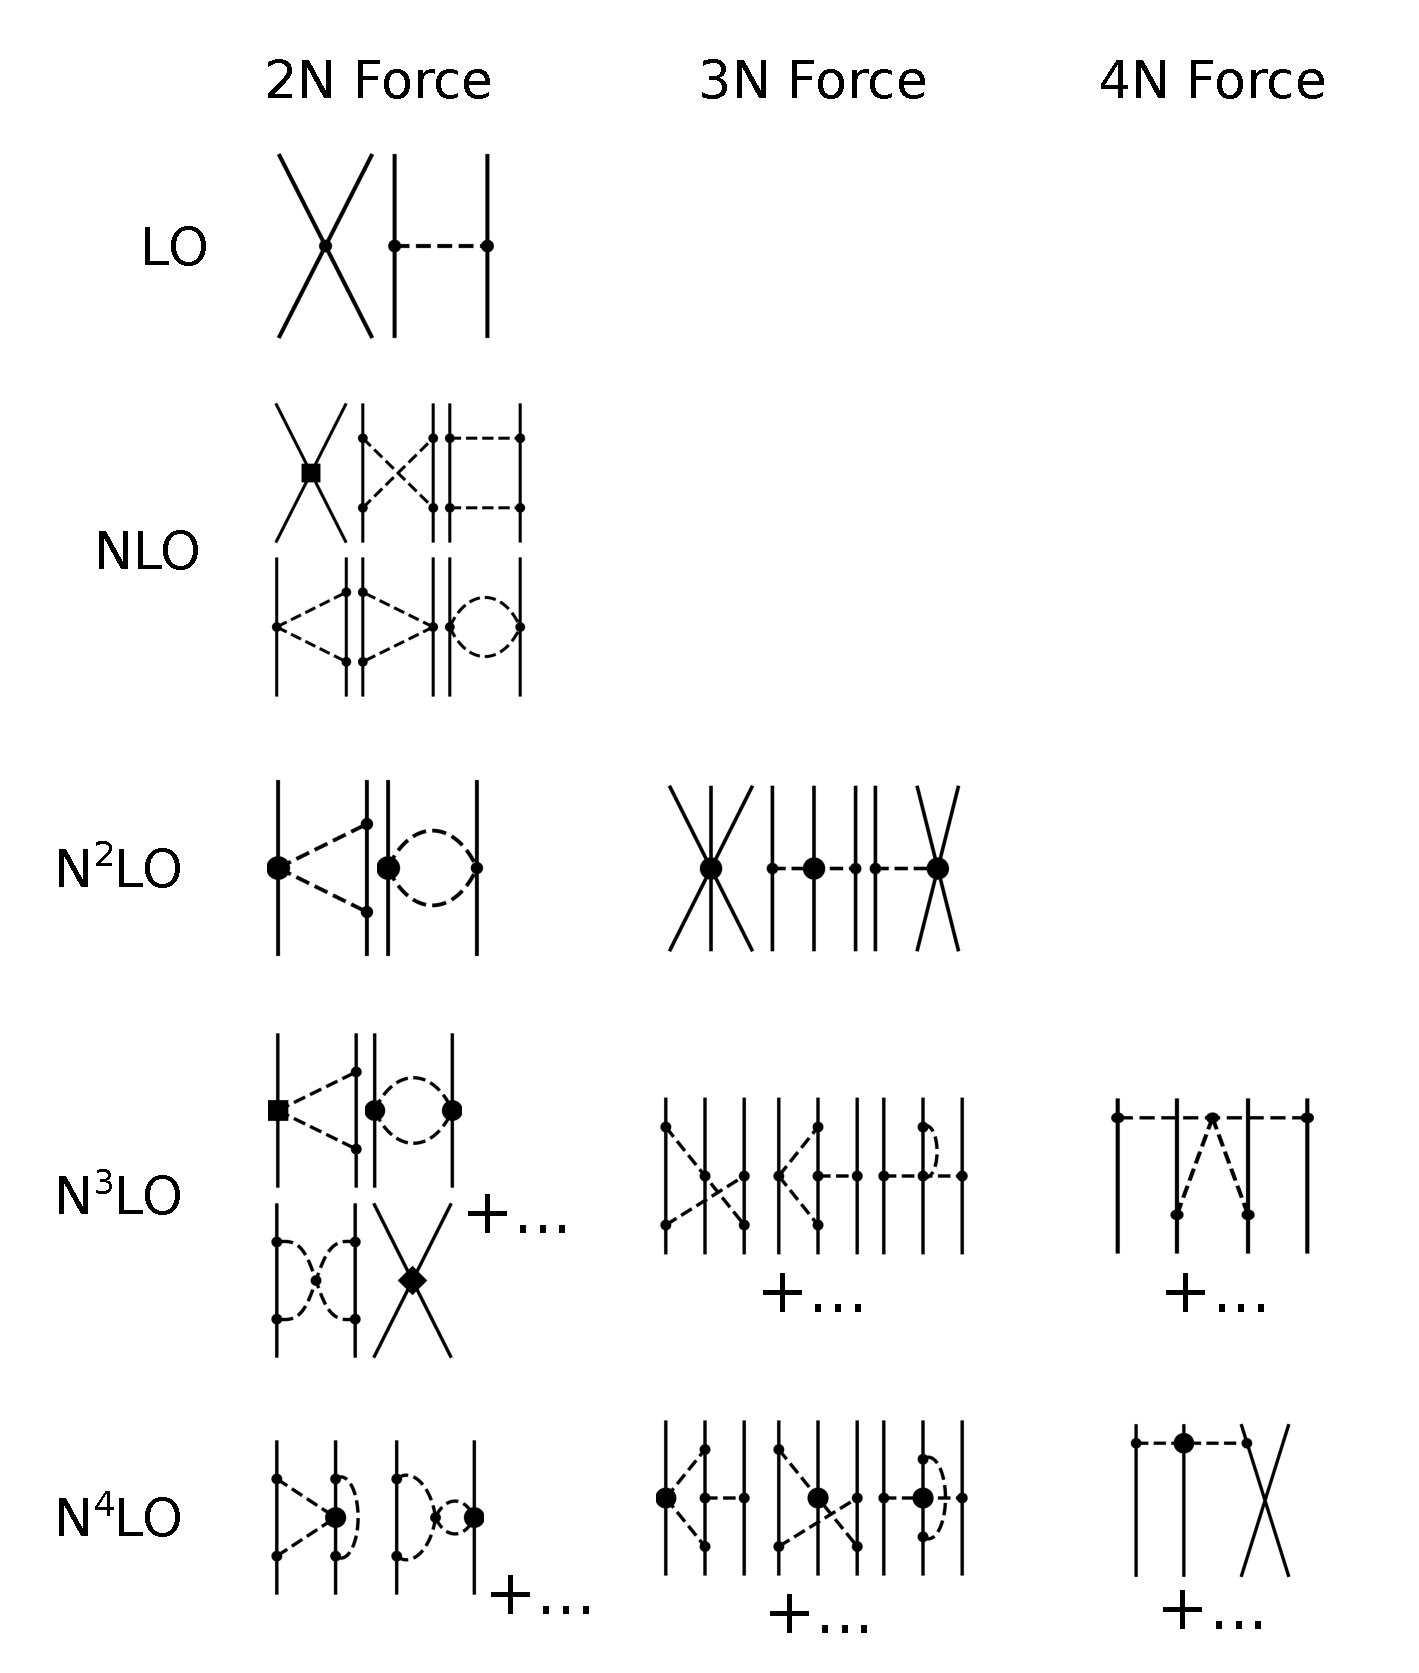
\includegraphics[width=0.6\textwidth]{Diagrams/Diagrams.pdf}
    \end{center}
    \caption{ Feynman diagrams for each of chiral orders and different nuclear forces (two-, three- and four-nucleon).
    Solid lines represent nucleons and dashed lines represent pions. Small dots, large solid dots,
    and diamonds denote different types of vertexes $\Delta_i$ (see \eq{powers} and \eq{Delta}).
    Further explanations are given e.g. in \cite{Entem2017}.}
    \label{chiral_diagrams}
\end{figure}

% \begin{figure}[h]
%     \begin{center}
%     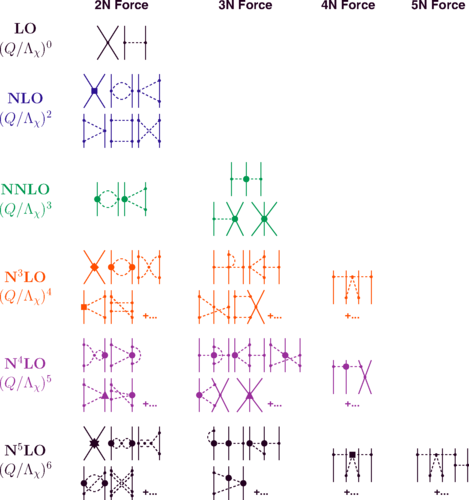
\includegraphics[width=0.6\textwidth]{Figures/chiral.png}
%     \end{center}
%     \caption{\tmp{To be removed}}
%     \label{chiral_diagrams}
% \end{figure}

The Argonne V18 potential \cite{AV18Wiringa}, mentioned earlier, has 40 adjustable parameters,
while \gls{ceft} NN potential at \gls{n4lo} \cite{Machleidt2011} has only 27 low-energy constants (LECs) fitted to 2N data.
The reduction of the number of free parameters of the \gls{ceft}-based potentials
has not only a theoretical but also a practical advantage in the studies of nuclear systems.

The general scheme outlined above was developed mainly by the Bochum-Bonn and Moscow-Idaho groups.
Both groups have similar approaches and were independently and almost simultaneously
developing their models. In 1998 Epelbaum and collaborators from the Bochum-Bonn group 
presented a first version of their \gls{nn} chiral potential \cite{EPELBAOUM1998107, epelbaum2000two}.
Developing more and more sophisticated versions with higher chiral orders, authors presented
in 2001 \cite{epelbaum_physrevc_2002} \gls{n2lo} model which included 3NF contributions,
and in 2005 \cite{epelbaum2005two} \gls{n3lo} NN potential.
They were further developing their chiral model, taking into account more Feynmann diagrams
coming to a higher chiral orders.
At some moment the Bochum-Bonn group faced a problem of potential regularization\cite{skibinski_3H, Witala_2014}.
Solving it was a necessary step but authors
were struggling with finding an appropriate
regularization method to handle the divergences that arise in the \gls{ceft} calculations.
Different techniques were applied such as the cutoff regularization and the regulator function methods.
An important step was made when authors started using a semi-local regularization 
in the coordinate space. The corresponding potential is called the \gls{scs} potential
(semi-local regularization in the coordinate space)\cite{Epelbaum2014SCS}.
% , see below in Sec{\temp{??}}.
Later similar regularization,
but done in momentum space was introduced, resulting in the most advanced chiral potential 
\cite{reinkrebs2018}: the \glsfirst{sms}. It is developed up to \gls{n4lo+} at the moment.

On the other side of the planet, in Idaho, R.~Machleidt and his group from Moscow(Ida\-ho) were also developing 
a chiral interaction. Their results from 2003 \cite{Entem2003}, following with later 
investigations \cite{Machleidt2005, Machleidt2010} and recently in \cite{Entem2017}
introduced a very similar model
to the one from the Bochum-Bonn group with minor technical differences.


There are a number of other attempts to construct the nuclear
potential from the \gls{ceft}.
% There are a number of another approaches within \gls{ceft} utilized.
% There are several other approaches within the framework of \gls{ceft}
% that have been utilized in nuclear physics.
M.Piarulli et al \cite{Piarulli2012,Piarulli2015} contributed
to quite a similar approach, based on
the same chiral potentials but including explicitly 
$\Delta$-isobar intermediate states 
up to the third chiral order and taking into account
sophisticated electromagnetic corrections.

Other groups try to improve already derived forces.
Let us mention here works by A.~Ekstr\"om and
collaborators \cite{ekstrom_2015, Tews_2020} who,
by using advanced fitting methods combined with
the statistical analysis proposed a so-called optimized interaction
V$_\text{opt}$ which was proved to provide a good description
of nuclei properties and nuclear matter without using 3NF.


Another approach is the pionless effective field
theory, which integrates pions out and
focuses on the various types of contact
interactions between nucleons \cite{hammer_review}.
Obtained potential has a very simple form, but cannot be applied
to higher energies since pions start playing an important role
there.

Yet another promising approach is the Lattice Effective Field Theory (LEFT), which
is based on the Lattice simulations of the strong
interaction. U.-G.~Mei\ss{}ner and collaborators have developed a chiral effective
theory for nuclear forces based on the methods of lattice QCD
calculations \cite{Lande2019}. This approach has the advantage of being able
to predict the nuclear force directly from the first
principles, without the need for phenomenological input. However, currently, it is limited
to small systems and low energies due to the computational
resources required for calculations.
Up to now, the relatively simple two-nucleon scattering problem
and few-nucleon bound state
have been solved within the LEFT and more complex systems are
still under attack. 
For more details please refer to
\cite{Lande2019}.


% {\color{red} Machleidt, Ekstr\"om, pion-less EFT, Lattice EFT(Mesissner), Girlanda, Piarulli}


Technically, the chiral potential may be derived both in coordinate and momentum spaces.
Nevertheless, in both cases, it requires regularization which 
improves potential behavior at small distances or at high momenta,
which allows to avoid infinities. 
% cuts 
% low coordinate values in order to avoid infinities 
% or high momentum values. 
The \gls{sms} potential is being regularized semilocally. 
It means that  local or nonlocal regularizations
are being applied for different parts of the potential.
% and later in \cite{Entem2017, Epelbaum2014SCS}
In \cite{Entem2003, epelbaum2005two} the non-local regulation scheme 
was applied to both short- and long-range parts
 of the potential while in the next model \cite{Entem2017, Epelbaum2014SCS}
 it affected only a short-range part. 
This regularization is applied directly to the potential matrix elements 
in the coordinate space:

\begin{equation}
    V_\pi(\vec{r}) \rightarrow V_{\pi,R} (\vec{r}) = V_\pi (\vec{r}) \left(1 - \exp(-r^2/R^2 )\right),
    \label{scs_regulator} 
\end{equation}
or in the momentum space

\begin{equation}
    V_\pi(\pvec{p}, \vec{p}) \rightarrow V_{\Lambda} (\pvec{p}, \vec{p}) = 
    V_\pi (\pvec{p}, \vec{p}) 
    \exp\left[-(p^\prime/\Lambda)^{2n} -(p/\Lambda)^{2n} \right],
    \label{sms_regulator} 
\end{equation}
where the cutoff R was chosen in the range of R = 0.8, ..., 1.2 \unit{fm},
$\Lambda = \frac{2}{R}$ and $n$ being adjusted with respect to the considered chiral order.
For specific case of the \gls{sms} force $\Lambda = \SIrange[range-phrase=-]{400}{550}{\mev}$ and $n=3$.

The other way of regularization, the local one, is applied to the propagator operator,
already during the derivation of potential. Namely, the Gaussian form factor $F(\vec{l}^2)$ is being used
to reduce pions with higher momenta:

\begin{equation}
    \int_{-\infty}^{\infty} \frac{\rho(\mu^2)}{\vec{l}^2 + \mu^2} d\mu^2 \rightarrow 
    \frac{F(\vec{l}^2)}{\vec{l}^2 + \mu^2}
\end{equation}
with

\begin{equation}
    F(\vec{l}^2) = e^{-\frac{\vec{l}^2 + M_\pi^2}{\Lambda^2}},
    \label{regulator}
\end{equation}
$M_\pi$ is an effective pion mass, $\Lambda$ - a cutoff parameter and $l$ is a four-momentum of the exchanged pion.
% \tmp{Further $\mu$ is a ...}
The form factor (\ref{regulator}), being used together with the Feynman propagator,
ensures that the long-range part of the forces has no singularities. 

The cut-off parameter $\Lambda$ is not fixed and usually calculations
are being performed for its different values. The comparison
of such results may reveal stronger or weaker dependence on $\Lambda$ and in a perfect
case, which is expected at $\nu >> 1$, one will come up with such a potential, where the cut will
not affect results at all. One of the aims of my thesis is to test how big cut-off dependency
of predictions is
observed for the \gls{sms} force.
To illustrate a cutoff dependency of the potential, in \fig{potential_cutoff} 
I show values of the matrix elements for 2N $\matrixel{p}{V}{p^\prime}$ potential $^3S_1-^3D_1$
as a function of the momentum $|\vec{p}|$ with fixed value $|\pvec{p}|$=\SI{1.798}{fm^{-1}}.
Please note, that the relatively strong dependency of specific matrix elements on the potential
is not always leading to a strong dependency of observables, as 
observables comprise contributions from many matrix elements.



\begin{figure}[htb]
    \begin{center}
    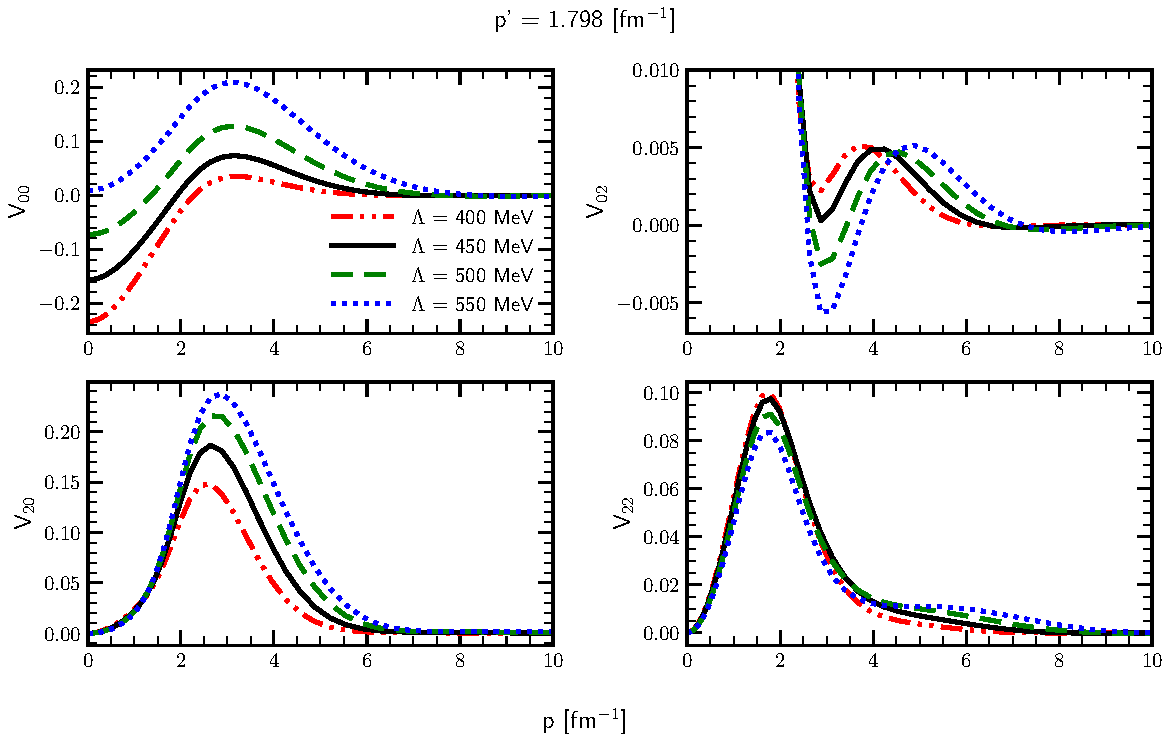
\includegraphics[width=0.95\textwidth]{PlotData/Deuteron/WAVEFUNC/potential_pp1.798.pdf}
    \end{center}
    \caption{Matrix elements $\matrixel{p}{V}{p^\prime}$ of the \gls{sms} potential in
    coupled partial waves $^3S_1 - ^3D_1$ as a function on the momentum $p$ with fixed
    value of the momentum $p'=\SI{1.798}{fm^{-1}}$. Potential element $V_{ll'}$
    is taken between two states with angular momenta  $l$ and $l'$ where $l=0$
    stands  for $^3S_1$ state and $l=2$ for $^3D_1$. 
    }
    \label{potential_cutoff}
\end{figure}


Let me add, that regularization function used by R.~Machleidt and collaborators 
is non-local only \cite{Entem2003, Entem2017}.
That is the main reason for the observed differences between predictions based on Epelbaum's
and Machleidt's models. 

\subsection*{Currents}


The electromagnetic current operator for a few-nucleon system has both one- and many-body contributions, which
can be denoted as $j_\mu^1$, $j_\mu^2$, $j_\mu^3$, etc, respectively 
(where $\mu = 0..3$ denotes a four-vector components).
The leading one-body contribution,
$j_\mu^1$, represents the photon's interaction with a single nucleon. The many-body contributions are known as
meson exchange currents (MEC) and arise from the meson-exchange picture of the nucleon-nucleon (NN)
interaction. 
In that picture, the photon can couple also to mesons exchanged between two nucleons, leading to two-body contributions to
the nuclear current.
The necessity of introducing the MEC arises from the continuity equation.
The momentum and isospin-dependent terms 
in the potential require the introduction of two-body MEC.
Similarly, the inclusion of the three-body force into the Hamiltonian requires the
existence of three-body contributions to the nuclear current. However, the effects of the three-body MEC are
likely negligible in the low-energy region.
Therefore, in the thesis, I will consider one- and two-body currents, only.
The continuity equation, connecting the interaction and the current clearly shows 
that those two quantities should be derived consistently from the same underlying theory
of nuclear phenomena.
I work with the \gls{sms} chiral interaction and for that force the complete consistent MEC
has not been derived yet.
Consistency includes here also the same regularization as used for the interaction.
While the derivation of such currents is ongoing \cite{krebs_private}, at the moment
only SNC is well established.
Thus to mimic the effects of the MEC, I apply the Siegert theorem \cite{Siegert, GolakKamad2000_ExplDescr}.
In general, this theorem allows the substitution of explicit MEC terms by the time component of the nuclear current (the charge density).
It is less sensitive to MEC contributions (compared to spatial components of $j_\mu$)
and thus in its case, the SNC approximation is sufficient.
I use here the formulation of the Siegert theorem given in \cite{GolakKamad2000_ExplDescr}.

A more detailed discussion of electromagnetic currents and pion absorption operators used here is given 
in the Sections~\ref{sec_current} and \ref{sec:pion_formalism}, respectively.


% There are several types of nuclear currents used for studying scattering processes. One of the most common types is the one-body current, which describes the motion of individual nucleons within the nucleus. This type of current can be further divided into two categories: the convection current and the spin current. The convection current is associated with the motion of the center of mass of the nucleus, while the spin current is associated with the intrinsic spin of the nucleons.

% Another important type of nuclear current is the two-body current, which describes the interaction between two nucleons within the nucleus. The two-body current is typically associated with meson exchange between the nucleons, and it plays a crucial role in scattering processes at low energies.

% A third type of nuclear current is the three-body current, which describes the interaction between three nucleons within the nucleus. This type of current is particularly important for studying scattering processes involving light nuclei, such as helium-3 or tritium.

% The use of nuclear currents in scattering experiments is essential for understanding the structure of the nucleus and the interactions between its constituent nucleons. Advances in theoretical and experimental techniques have allowed for more precise measurements of these currents and have provided insights into the fundamental properties of the nucleus.
